\documentclass[../../../main.tex]{subfiles}

%Break lines: 
% - In Neville's algorithm (section: interpolation -polynomial interpolation)
% - In Newton-Raphson modified method (section: zeros of functions-root_finding methods)
\begin{document}
\begin{multicols}{2}[\section{Numerical methods}]
\subsection{Errors}
\subsubsection*{Floating-point representation}
\begin{theorem}
    Let $b\in\mathbb{N}$, $b\geq 2$. Any real number $x\in\mathbb{R}$ can be represented of the form 
    \begin{equation*}
        x=s\left(\sum_{i=1}^\infty\alpha_ib^{-i}\right)b^q,
    \end{equation*} where $s\in\{-1,1\}$, $q\in\mathbb{Z}$ and $\alpha_i\in\{0,1,\ldots,b-1\}$. Moreover, this representation is unique if $\alpha_1\ne0$ and $\forall i_0\in\mathbb{N}$, $\exists i\geq i_0:\alpha_i\ne b-1$. We will write $$x=s(0.\alpha_1\alpha_2\cdots)_bb^q,$$ where the subscript $b$ in the parenthesis indicates that the number $0.\alpha_1\alpha_2\alpha_3\cdots$ is in base $b$.
\end{theorem}
\begin{definition}[Floating-point representation]
    Let $x$ be a real number. Then the floating-point representation of $x$ is $$x=s\left(\sum_{i=1}^t\alpha_ib^{-i}\right)b^q.$$ Here $s$ is called the \textit{sign}; $\sum_{i=1}^t\alpha_ib^{-i}$, the \textit{significant} or \textit{mantissa}, and $q$, the \textit{exponent}, limited to a prefixed range $q_\text{min}\leq q\leq q_\text{max}$. So, the floating-point representation of $x$ is $$x=smb^q=s(0.\alpha_1\alpha_2\cdots\alpha_t)_bb^q.$$ Finally we say a floating-point number is \textit{normalized} if $\alpha_1\ne0$.
\end{definition}
\begin{table}[ht]
    \centering
    \begin{tabular}{c|ccccc}
        Format & $b$ & $t$ & $q_\text{min}$ & $q_\text{max}$ & bits \\
        \hline\hline
        IEEE simple & 2 & 24 & -126 & 127 & 32\\
        IEEE double & 2 & 53 & -1022 & 1023 & 64
    \end{tabular}
    \caption{Parameters of IEEE simple and IEEE double formats.}
    \label{tab:my_label}
\end{table}
\begin{definition}
    Let $x\in\mathbb{R}$ be such that $x=s(0.\alpha_1\alpha_2\cdots)_bb^q$ with $q_\text{min}\leq q\leq q_\text{max}$. We say the \textit{floating-point representation by truncation of $x$} is $$fl_T(x)=s(0.\alpha_1\alpha_2\cdots\alpha_t)_bb^q.$$ We say the \textit{floating-point representation by rounding of $x$} is
    \begin{multline*}
        fl_R(x)=\\=\left\{\text{\setlength{\tabcolsep}{4pt}\begin{tabular}{m{3.85cm}m{3cm}}
            $s(0.\alpha_1\cdots\alpha_t)_bb^q$ & if $\ 0\leq\alpha_{t+1}<\frac{b}{2}$\\
            $s(0.\alpha_1\cdots\alpha_{t-1}(\alpha_t+1))_bb^q$ & if $\ \frac{b}{2}\leq\alpha_{t+1}\leq b-1.$
        \end{tabular}}\right.
    \end{multline*}
\end{definition}
\begin{definition}
    Given a value $x\in\mathbb{R}$ and an approximation $\Tilde{x}$ of $x$, the \textit{absolute error} is $$\Delta x:=|x-\Tilde{x}|.$$ If $x\ne 0$, the \textit{relative error} is $$\delta x:=\frac{|x-\Tilde{x}|}{x}.$$ If $x$ is unknown, we take $$\delta x\approx\frac{|x-\Tilde{x}|}{\Tilde{x}}.$$
\end{definition}
\begin{definition}
    Let $\Tilde{x}$ be an approximation of $x$. If $\Delta x\leq\frac{1}{2}10^{-t}$, we say \textit{$\Tilde{x}$ has $t$ correct decimal digits}. If $x=sm10^q$ with $0.1\leq m<1$, $\Tilde{x}=s\Tilde{m}10^q$ and $$u:=\max\{i\in\mathbb{Z}:|m-\Tilde{m}|\leq\frac{1}{2}10^{-i}\},$$ then we say that $\Tilde{x}$ \textit{has $u$ significant digits}.
\end{definition}
\begin{prop}
    Let $x\in\mathbb{R}$ be such that $x=s(0.\alpha_1\alpha_2\cdots)_bb^q$ with $\alpha_1\ne0$ and $q_\text{min}\leq q\leq q_\text{max}$. Then, its floating-point representation in base $b$ and with $t$ digits satisfy:
    \begin{align*}
        \left|fl_T(x)-x\right|\leq b^{q-t},\quad&\quad \left|fl_R(x)-x\right|\leq\frac{1}{2}b^{q-t}.\\
        \left|\frac{fl_T(x)-x}{x}\right|\leq b^{1-t},\quad&\quad \left|\frac{fl_R(x)-x}{x}\right|\leq\frac{1}{2}b^{1-t}.
    \end{align*}
\end{prop}
\begin{definition}
    The \textit{machine epsilon $\epsilon$} is defined as $$\epsilon:=\min\{\varepsilon>0:fl(1+\varepsilon)\ne 1\}.$$
\end{definition}
\begin{prop}
    For a machine working by truncation, $\epsilon=b^{1-t}$. For a machine working by rounding, $\epsilon=\frac{1}{2}b^{1-t}$.
\end{prop}
\subsubsection*{Propagation of errors}
\begin{prop}[Propagation of absolute errors]
    Let $f:\mathbb{R}^n\rightarrow\mathbb{R}$ be a function of class $\mathcal{C}^2$. If $\Delta x_j$ is the absolute error of the variable $x_j$ and $\Delta f(x)$ is the absolute error of the function $f$ evaluated at the point $x=(x_1,\ldots,x_n)$, we have $$|\Delta f(x)|\lesssim\sum_{j=1}^n\left|\frac{\partial f}{\partial x_j}(x)\right||\Delta x_j|\footnote{The symbol $\lesssim$ means that we are omitting terms of order $\Delta x_j\Delta x_k$ and higher.}.$$ The coefficients $\left|\frac{\partial f}{\partial x_j}(x)\right|$ are called \textit{absolute condition numbers of the problem}. 
\end{prop}
\begin{prop}[Propagation of relative errors]
    Let $f:\mathbb{R}^n\rightarrow\mathbb{R}$ be a function of class $\mathcal{C}^2$. If $\delta x_j$ is the relative error of the variable $x_j$ and $\delta f(x)$ is the relative error of the function $f$ evaluated at the point $x=(x_1,\ldots,x_n)$, we have $$|\delta f(x)|\lesssim\sum_{j=1}^n\frac{\left|\frac{\partial f}{\partial x_j}(x)\right|\left|x_j\right|}{\left|f(x)\right|}|\delta x_j|.$$ The coefficients $\frac{\left|\frac{\partial f}{\partial x_j}(x)\right|\left|x_j\right|}{\left|f(x)\right|}$ are called \textit{relative condition numbers of the problem}. 
\end{prop}
\subsubsection*{Numerical stability of algorithms}
\begin{definition}
    An algorithm is said to be \textit{numerically stable} if  errors in the input lessen in significance as the algorithm executes, having little effect on the final output. On the other hand, an algorithm is said to be \textit{numerically unstable} if errors in the input cause a considerably larger error in the final output.
\end{definition}
\begin{definition}
    A problem with a low condition number is said to be \textit{well-conditioned}. Conversely, a problem with a high condition number is said to be \textit{ill-conditioned}.
\end{definition}
\subsection{Zeros of functions}
\begin{definition}
    Let $f:\mathbb{R}\rightarrow\mathbb{R}$ be a function. We say $\alpha$ is a \textit{zero} or a \textit{solution to the equation $f(x)=0$} if $f(\alpha)=0$.
\end{definition}
\begin{definition}
    Let $f:\mathbb{R}\rightarrow\mathbb{R}$ be a sufficiently differentiable function. We say $\alpha$ is a \textit{zero of multiplicity $m\in\mathbb{N}$} if $$f(\alpha)=f'(\alpha)=\cdots=f^{(m-1)}(\alpha)=0\quad\text{and}\quad f^{(m)}(\alpha)\ne0.$$ If $m=1$, the zero is called \textit{simple}; if $m=2$, \textit{double}; if $m=3$, \textit{triple}...
\end{definition}
\subsubsection*{Root-finding methods}
    For the following methods consider a continuous function $f:I\subseteq\mathbb{R}\rightarrow\mathbb{R}$ with an unknown zero $\alpha\in I$. Given $\varepsilon>0$, we want to approximate $\alpha$ with $\Tilde{\alpha}$ such that $|\alpha-\Tilde{\alpha}|<\varepsilon$.
\begin{theorem}[Bisection method]
    Suppose $I=[a_0,b_0]$. For each step $n\geq 0$ of the algorithm we will approximate $\alpha$ by $$c_n=\frac{a_n+b_n}{2}.$$ If $f(c_n)=0$ we are done. If not, let 
    $$[a_{n+1},b_{n+1}]=\left\{
    \begin{array}{ccc}
        [a_n,c_n] & \text{if} & f(a_n)f(c_n)<0, \\
        \left[c_n,b_n\right] & \text{if} & f(a_n)f(c_n)>0.
    \end{array}\right.$$ 
    and iterate the process again\footnote{Note that bisection method only works for zeros of odd multiplicity.}. Observe the length of the interval $[a_n,b_n]$ is $\frac{b_0-a_0}{2^n}$ and therefore: $$|\alpha-c_n|<\frac{b_0-a_0}{2^{n+1}}<\varepsilon\iff n>\frac{\log\left(\frac{b_0-a_0}{\varepsilon}\right)}{\log 2}-1.$$
\end{theorem}
\begin{theorem}[\textit{Regula falsi} method]
    Suppose $I=[a_0,b_0]$. For each step $n\geq 0$ of the algorithm we will approximate $\alpha$ by $$c_n=b_n-f(b_n)\frac{b_n-a_n}{f(b_n)-f(a_n)}=\frac{a_nf(b_n)-b_nf(a_n)}{f(b_n)-f(a_n)}.$$ If $f(c_n)=0$ we are done. If not, let
    $$[a_{n+1},b_{n+1}]=\left\{
    \begin{array}{ccc}
        [a_n,c_n] & \text{if} & f(a_n)f(c_n)<0, \\
        \left[c_n,b_n\right] & \text{if} & f(a_n)f(c_n)>0,
    \end{array}\right.$$ 
    and iterate the process again.
\end{theorem}
\begin{theorem}[Secant method]
    Suppose $I=\mathbb{R}$ and that we have two different initial approximations $x_0$, $x_1$. Then for each step $n\geq 0$ of the algorithm we obtain a new approximation $x_{n+2}$, given by: $$x_{n+2}=x_{n+1}-f(x_{n+1})\frac{x_{n+1}-x_n}{f(x_{n+1})-f(x_n)}.$$
\end{theorem}
\begin{theorem}[Newton-Raphson method]
    Suppose $I=\mathbb{R}$, $f\in\mathcal{C}^1$ and that we have an initial approximation $x_0$. Then for each step $n\geq 0$ we obtain a new approximation $x_{n+1}$, given by: $$x_{n+1}=x_n-\frac{f(x_n)}{f'(x_n)}.$$
\end{theorem}
\begin{theorem}[Newton-Raphson modified\\method]
    Suppose $I=\mathbb{R}$, $f\in\mathcal{C}^1$ and that we have an initial approximation $x_0$ of a zero $\alpha$ of multiplicity $m$. Then for each step $n\geq 0$ we obtain a new approximation $x_{n+1}$, given by: $$x_{n+1}=x_n-m\frac{f(x_n)}{f'(x_n)}.$$
\end{theorem}
\begin{theorem}[Chebyshev method]
    Suppose $I=\mathbb{R}$, $f\in\mathcal{C}^2$ and that we have an initial approximation $x_0$. Then for each step $n\geq 0$ we obtain a new approximation $x_{n+1}$, given by: $$x_{n+1}=x_n-\frac{f(x_n)}{f'(x_n)}-\frac{1}{2}\frac{\left[f(x_n)\right]^2f''(x_n)}{\left[f'(x_n)\right]^3}.$$
\end{theorem}
\subsubsection*{Fixed-point iterations}
\begin{definition}
    Let $g:[a,b]\rightarrow[a,b]\subset\mathbb{R}$ be a function. A point $\alpha\in[a,b]$ is \textit{n-periodic} if $g^n(\alpha)=\alpha$ and $g^j(\alpha)\ne\alpha$ for $j=1,\ldots,n-1$\footnote{Note that 1-periodic points are the fixed points of $f$.}.
\end{definition}
\begin{theorem}[Fixed-point theorem]
    Let $(M,d)$ be a complete metric space and $g:M\rightarrow M$ be a contraction\footnote{Remember definitions \ref{FOSV_metric}, \ref{FOSV_complete} and \ref{FOSV_contr}.}. Then $g$ has a unique fixed point $\alpha\in M$ and for every $x_0\in M$, $$\lim_{n\to\infty}x_n=\alpha,\quad\text{where }x_n=g(x_{n-1})\quad\forall n\in\mathbb{N}.$$
\end{theorem}
\begin{prop}
    Let $(M,d)$ be a metric space and $g:M\rightarrow M$ be a contraction of constant $k$. Then if we want to approximate a fixed point $\alpha$ by the iteration $x_n=g(x_{n-1})$, we have:
    \begin{align*}
        d(x_n,\alpha)&\leq\frac{k^n}{1-k}d(x_1,x_0)\quad&\text{(a priori estimation)}\\
        d(x_n,\alpha)&\leq\frac{k}{1-k}d(x_n,x_{n-1})\quad&\text{(a posteriori estimation)}
    \end{align*}
\end{prop}
\begin{corollary}
    Let $g:\mathbb{R}\rightarrow\mathbb{R}$ be a function of class $\mathcal{C}^1$. Suppose $\alpha$ is a fixed point of $g$ and $|g'(\alpha)|<1$. Then, there exists $\varepsilon>0$ and $I_\varepsilon:=[\alpha-\varepsilon,\alpha+\varepsilon]$ such that $g(I_\varepsilon)\subseteq I_\varepsilon$ and $g$ is a contraction on $I_\varepsilon$. In particular, if $x_0\in I_\varepsilon$, the iteration $x_{n+1}=g(x_n)$ converges to $\alpha$.
\end{corollary}
\begin{definition}
    Let $g:\mathbb{R}\rightarrow\mathbb{R}$ be a function of class $\mathcal{C}^1$ and $\alpha$ be a fixed point of $g$. We say $\alpha$ is an \textit{attractor fixed point} if $|g'(\alpha)|<1$. In this case, any iteration $x_{n+1}=g(x_n)$ in $I_\varepsilon$ converges to $\alpha$. If $|g'(\alpha)|>1$, we say $\alpha$ is a \textit{repulsor fixed point}. In this case, $\forall x_0\in I_\varepsilon$ the iteration $x_{n+1}=g(x_n)$ doesn't converge to $\alpha$.
\end{definition}
\begin{center}
    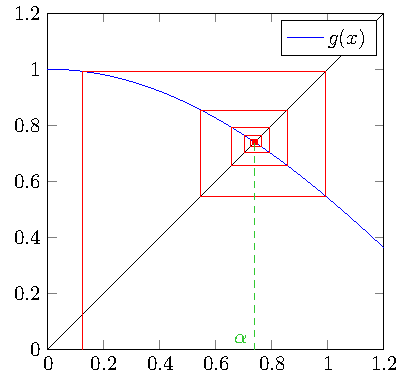
\includegraphics[width=0.49\linewidth]{Images/cobweb1.tex}\hfill
    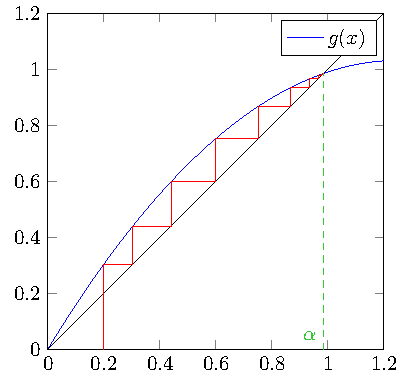
\includegraphics[width=0.49\linewidth]{Images/cobweb2.tex}\\
    \vspace{0.02\linewidth}
    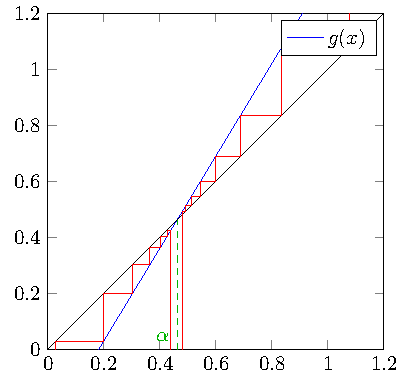
\includegraphics[width=0.49\linewidth]{Images/cobweb3.tex}\hfill
    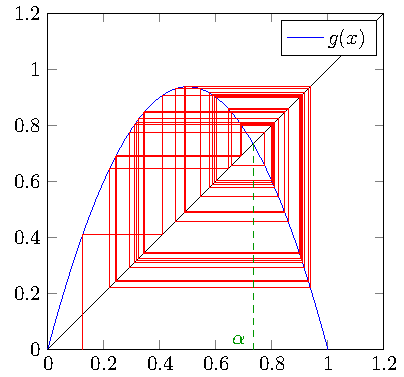
\includegraphics[width=0.49\linewidth]{Images/cobweb4.tex}
    \captionof{figure}{Cobweb diagrams. In the figures at the top, $\alpha$ is a attractor point, that is, $|g'(\alpha)|<1$. More precisely, the figure at the top left occurs when $-1<g'(\alpha)\leq0$ and the figure at the top right when $0\leq g'(\alpha)<1$. In the figure at bottom left, $\alpha$ is a repulsor point. Finally, in the figure at bottom right the iteration $x_{n+1}=g(x_n)$ has no limit. It is said that to have a \textit{chaotic behavior}.}
\end{center}
\subsubsection*{Order of convergence}
\begin{definition}[Order of convergence]
    Let $(x_n)$ be a sequence of real numbers that converges to $\alpha\in\mathbb{R}$. We say $(x_n)$ has \textit{order of convergence $p\in\mathbb{R}^+$} if exists $C>0$ such that: $$\lim_{n\to\infty}\frac{|x_{n+1}-\alpha|}{|x_n-\alpha|^p}=C.$$ The constant $C$ is called \textit{asymptotic error constant}. For the case $p=1$, we need $C<1$. In this case the convergence is called \textit{linear convergence}; for $p=2$, is called \textit{quadratic convergence}; for $p=3$, \textit{cubic convergence}... If it's satisfied that $$\lim_{n\to\infty}\frac{|x_{n+1}-\alpha|}{|x_n-\alpha|^p}=0$$ for some $p\in\mathbb{R}^+$, we say the sequence has \textit{order of convergence at least $p$}.
\end{definition}
\begin{theorem}
    Let $g:\mathbb{R}\rightarrow\mathbb{R}$ be a function of class $\mathcal{C}^p$ and let $\alpha$ be a fixed point of $g$. Suppose $$g'(\alpha)=g''(\alpha)=\cdots=g^{(p-1)}(\alpha)=0$$ with $|g'(\alpha)|<1$ if $p=1$. Then the iteration $x_{n+1}=g(x_n)$, with $x_0$ sufficiently close to $\alpha$, has order of convergence at least $p$. If, moreover, $g^{(p)}(\alpha)\ne0$, then the previous iteration has order of convergence $p$ with asymptotic error constant $C=\frac{|g^{(p)}(\alpha)|}{p!}$.
\end{theorem}
\begin{theorem}
    Let $f:\mathbb{R}\rightarrow\mathbb{R}$ be a function of class $\mathcal{C}^3$ and $\alpha$ be a simple zero of $f$. If $f''(\alpha)\ne0$, then Newton-Raphson method for finding $\alpha$ has quadratic convergence with asymptotic error constant $C=\frac{1}{2}\left|\frac{f''(\alpha)}{f'(\alpha)}\right|$.\par If $f\in\mathcal{C}^{m+2}$, and $\alpha$ is a zero of multiplicity $m>1$, then Newton-Raphson method has linear convergence but Newton-Raphson modified method has at least quadratic convergence.
\end{theorem}
\begin{theorem}
    Let $f:\mathbb{R}\rightarrow\mathbb{R}$ be a function of class $\mathcal{C}^3$ and let $\alpha$ be a simple zero of $f$. Then Chebyshev's method for finding $\alpha$ has at least cubic convergence.
\end{theorem}
\begin{definition}
    We define the \textit{computational efficiency of an algorithm} as a function $E(p,t)$, where $t$ is the time taken for each iteration of the method and $p$ is the order of convergence of the method. $E(p,t)$ must satisfy the following properties:
    \begin{enumerate}
        \item $E(p,t)$ is increasing with respect to the variable $p$ and decreasing with respect to $t$.
        \item $E(p,t)=E(p^m,mt)$ $\forall m\in\mathbb{R}$.
    \end{enumerate}
    Examples of such functions are the following: $$E(p,t)=\frac{\log p}{t},\quad E(p,t)=p^{1/t}.$$
\end{definition}
\subsubsection*{Sequence acceleration}
\begin{definition}[Aitken's $\Delta^2$ method]
    Let $(x_n)$ be a sequence of real numbers. We denote:
    \begin{gather*}
        \Delta x_n:=x_{n+1}-x_n,\\\Delta^2 x_n:=\Delta x_{n+1}-\Delta x_n=x_{n+2}-2x_{n+1}+x_n.
    \end{gather*}
    \textit{Aitken's $\Delta^2$ method} is the transformation of the sequence $(x_n)$ into a sequence $y_n$, defined as: $$y_n:=x_n-\frac{(\Delta x_n)^2}{\Delta^2 x_n}=x_n-\frac{(x_{n+1}-x_n)^2}{x_{n+2}-2x_{n+1}+x_n},$$ with $y_0=x_0$.
\end{definition}
\begin{theorem}
    Let $(x_n)$ be a sequence of real numbers such that $\displaystyle\lim_{n\to\infty}x_n=\alpha$, $x_n\ne\alpha$ $\forall n\in\mathbb{N}$ and $\exists C$, $|C|<1$, satisfying $$x_{n+1}-\alpha=(C+\delta_n)(x_n-\alpha),\quad\text{with }\lim_{n\to\infty}\delta_n=0.$$ Then the sequence $(y_n)$ obtained from Aitken's $\Delta^2$ process is well-defined and $$\lim_{n\to\infty}\frac{y_n-\alpha}{x_n-\alpha}=0\footnote{This means that Aitken's $\Delta^2$ method produces an acceleration of the convergence of the sequence $(x_n)$.}.$$
\end{theorem}
\begin{theorem}[Steffensen's method]
    Let $g:\mathbb{R}\rightarrow\mathbb{R}$ be a continuous function and suppose we have an iterative method $x_{n+1}=g(x_n)$. Then for each step $n$ we can consider a new iteration $y_{n+1}$, with $y_0=x_0$, given by: $$y_{n+1}=y_n-\frac{\left(g(y_n)-y_n\right)^2}{g(g(y_n))-2g(y_n)+y_n}.$$
\end{theorem}
\begin{prop}
    Let $f:\mathbb{R}\rightarrow\mathbb{R}$ be a function of class $\mathcal{C}^2$ and $\alpha$ be a simple zero of $f$. Then Steffensen's method for finding $\alpha$ has at least quadratic convergence\footnote{Note that the advantage of Steffensen's method over Newton-Raphson method is that in the former we don't need the differentiability of the function whereas in the latter we do.}.
\end{prop}
\subsubsection*{Zeros of polynomials}
\begin{lemma}
    Let $p(z)=a_0+a_1z+\cdots+a_nz^n\in\mathbb{C}[x]$ with $a_n\ne 0$. We define $$\lambda:=\max\left\{\left\|\frac{a_i}{a_n}\right\|:i=0,1,\ldots,n-1\right\}.$$ Then if $p(\alpha)=0$ for some $\alpha\in\mathbb{C}$, $\|\alpha\|\leq\lambda+1$.
\end{lemma}
\begin{definition}[Strum's sequence]
    Let $(f_i)$, $i=0,\ldots,n$, be a sequence of continuous functions defined on $[a,b]\subset\mathbb{R}$ and $f:[a,b]\rightarrow\mathbb{R}$ be a function of class $\mathcal{C}^1$ such that $f(a)f(b)\ne 0$. We say $(f_n)$ is a \textit{Sturm's sequence} if:
    \begin{enumerate}
        \item $f_0=f$.
        \item If $\alpha\in[a,b]$ satisfies $f_0(\alpha)=0\implies f_0'(\alpha)f_1(\alpha)>0$.
        \item For $i=1,\ldots,n-1$, if $\alpha\in[a,b]$ satisfies $f_i(\alpha)=0\implies f_{i-1}(\alpha)f_{i+1}(\alpha)<0$.
        \item $f_n(x)\ne0$ $\forall x\in[a,b]$.
    \end{enumerate}
\end{definition}
\begin{definition}
    Let $(a_i)$, $i=0,\ldots,n$, be a sequence. We define $\nu(a_i)$ as the number of sign variations of the sequence $$\{a_0,a_1,\ldots,a_n\},$$ without taking into account null values. 
\end{definition}
\begin{theorem}[Sturm's theorem]
    Let $f:[a,b]\rightarrow\mathbb{R}$ be a function of class $\mathcal{C}^1$ such that $f(a)f(b)\ne 0$ and with a finite number of zeros. Let $(f_i)$, $i=0,\ldots,n$, be a Sturm sequence defined on $[a,b]$. Then the number of zeros of $f$ on $[a,b]$ is $$\nu\left(f_i(a)\right)-\nu\left(f_i(b)\right).$$
\end{theorem}
\begin{lemma}
    Let $p\in\mathbb{C}[x]$ be a polynomial. Then the polynomial $\displaystyle q=\frac{p}{\gcd(p,p')}$ has the same roots as $p$ but all of them are simple.
\end{lemma}
\begin{prop}
    Let $p\in\mathbb{R}[x]$ be a polynomial with $\deg p=m$. We define $\displaystyle f_0=\frac{p}{\gcd(p,p')}$ and $f_1=f_0'$. If $\deg f_0=n$, then for $i=0,1,\ldots,n-2$, we define $f_{i+2}$ as $$f_i(x)=q_{i+1}(x)f_{i+1}(x)-f_{i+2}(x),$$ (similarly to the euclidean division between $f_i$ and $f_{i+1}$). Then $f_n$ is constant and hence the sequence $(f_i)$, $i=0,\ldots,n$, is a Sturm sequence.
\end{prop}
\begin{theorem}[Budan-Fourier theorem]
    Let $p\in\mathbb{R}[x]$ be a polynomial with $\deg p=n$. Consider the sequence $(p^{(i)})$, $i=0,\ldots,n$. If $p(a)p(b)\ne 0$, the number of zeros of $p$ on $[a,b]$ is $$\nu\left(p^{(i)}(a)\right)-\nu\left(p^{(i)}(b)\right)-2k,\quad\text{for some }k\in\mathbb{N}\cup\{0\}.$$
\end{theorem}
\begin{corollary}[Descartes' rule of signs]
    Let $p=a_0+a_1x+\cdots+a_nx^n\in\mathbb{R}[x]$ be a polynomial. If $p(0)\ne 0$, the number of zeros of $p$ on $[0,\infty)$ is $$\nu(a_i)-2k,\quad\text{for some }k\in\mathbb{N}\cup\{0\}\footnote{Note that making the change of variable $t=-x$ one can obtain the number of zeros on $(-\infty,0]$ of $p$ by considering the polynomial $p(t)$.}.$$
\end{corollary}
\begin{theorem}[Greshgorin theorem]
    Let $A=(a_{ij})\in\mathcal{M}_n(\mathbb{C})$ be a complex matrix and $\lambda$ be an eigenvalue of $A$. For all $i,j\in\{1,2,\ldots,n\}$ we define:
    \begin{gather*}
        r_i=\sum_{\substack{k=1\\k\ne i}}^n|a_{ik}|,\quad R_i=\{z\in\mathbb{C}:|z-a_{ii}|\leq r_i\},\\
        c_j=\sum_{\substack{k=1\\k\ne j}}^n|a_{kj}|,\quad C_j=\{z\in\mathbb{C}:|z-a_{jj}|\leq c_j\}.
    \end{gather*}
    Then $\lambda\in\bigcup_{i=1}^nR_i$ and $\lambda\in\bigcup_{j=1}^nC_j$. Moreover in each connected component of $\bigcup_{i=1}^nR_i$ (respectively $\bigcup_{j=1}^nC_j$) there are as many eigenvalues (taking into account the multiplicity) as disks $R_i$ (respectively $C_i$).
\end{theorem}
\begin{corollary}
    Let $p(z)=a_0+a_1z+\cdots+a_nz^n+z^{n+1}\in\mathbb{C}[x]$. We define
    \begin{gather*}
        r=\sum_{i=1}^{n-1}|a_i|,\quad c=\max\{|a_0|,|a_1|+1,\ldots,|a_{n-1}|+1\}.
    \end{gather*}
    Then if $p(\alpha)=0$ for some $\alpha\in\mathbb{C}$, $$\alpha\in(B(0,1)\cup B(-a_n,r))\cap(B(-a_n,1)\cup B(0,c)).$$
\end{corollary}
\subsection{Interpolation}
\begin{definition}
    Suppose we have a family of real valued functions $\mathfrak{C}$ and a set of points $\{(x_i,y_i)\}_{i=0}^n:=\{(x_i,y_i)\in\RR^2:i=0,\ldots,n\text{ and }x_j\ne x_k\iff j\ne k\}$. These points $\{(x_i,y_i)\}_{i=0}^n$ are called \textit{support points}. The \textit{interpolation problem} consists in finding a function $f\in\mathfrak{C}$ such that $f(x_i)=y_i$ for $i=0,\ldots,n$\footnote{Types of interpolation are for example polynomial interpolation, trigonometric interpolation, Padé interpolation, Hermite interpolation and spline interpolation.}.
\end{definition}
\subsubsection*{Polynomial interpolation}
\begin{definition}
    Given a set of support points $\{(x_i,y_i)\}_{i=0}^n$, \textit{Lagrange's interpolation problem} consists in finding a polynomial $p_n\in\mathbb{R}[x]$ such that $\deg p_n\leq n$ and $p_n(x_i)=y_i$.
\end{definition}
\begin{definition}
    Let $\{(x_i,y_i)\}_{i=0}^n$ be a set of support points. We define $\omega_n(x)\in\RR[x]$ as $$\omega_n(x)=\prod_{k=0}^n(x-x_k).$$ We define \textit{Lagrange basis polynomials} $L_j(x)\in\RR[x]$ as $$L_j(x)=\frac{\omega_n(x)}{(x-x_j)\omega_n(x_j)}=\prod_{\substack{k=0\\k\ne j}}^n\frac{x-x_k}{x_j-x_k}.$$
\end{definition}
\begin{prop}
    Let $\{(x_i,y_i)\}_{i=0}^n$ be a set of support points. Then, Lagrange's interpolation problem has a unique solution and this is: $$p_n(x)=\sum_{i=0}^ny_iL_i(x).$$
\end{prop}
\begin{prop}[Neville's algorithm]
    Let \\$\{(x_i,y_i)\}_{i=0}^n$ be a set of support points, $\{i_0,\ldots,i_k\}\subset\{0,\ldots,n\}$ and $P_{i_1,\ldots,i_k}(x)\in\mathbb{R}[x]$ be such that $\deg P_{i_0,\ldots,i_k}\leq k$ and $P_{i_1,\ldots,i_k}(x_{i_j})=y_{i_j}$ for $j=0,\ldots,k$. Then, it is satisfied that:
    \begin{enumerate}
        \item $P_i(x)=y_i$.
        \item $P_{i_0,\ldots,i_k}(x)=\frac{\begin{vmatrix}
        P_{i_1,\ldots,i_k}(x) & x-x_{i_k}\\
        P_{i_0,\ldots,i_{k-1}}(x) & x-x_{i_0}
        \end{vmatrix}}{x_{i_k}-x_{i_0}}$
    \end{enumerate}
\end{prop}
\begin{definition}
    Let $f:\mathbb{R}\rightarrow\mathbb{R}$ be a function and $\{x_i\}_{i=0}^k\subset\mathbb{R}$ be pairwise distinct points. We define the \textit{divided difference of order $k$ of $f$ applied to $\{x_i\}_{i=0}^k$}, denoted by $f[x_0,\ldots,x_k]$, as the coefficient of $x^k$ of the interpolating polynomial with support points $\{(x_i,f(x_i))\}_{i=0}^k$ 
\end{definition}
\begin{prop}
    Let $f:\mathbb{R}\rightarrow\mathbb{R}$ be a function and $\{x_i\}_{i=0}^k\subset\mathbb{R}$ be different points. Lagrange interpolating polynomial with support points $\{(x_i,f(x_i))\}_{i=0}^n$ is $$p_n(x)=\sum_{j=0}^nf[x_0,\ldots,x_j]\omega_{j-1}(x),$$ assuming $\omega_{-1}:=1$.
\end{prop}
\begin{prop}[Newton's divided differences method]
    Let $f:\mathbb{R}\rightarrow\mathbb{R}$ be a function. For $x\in\mathbb{R}$, we have $f[x]=f(x)$. And if $\{x_i\}_{i=0}^n\subset\mathbb{R}$ are different points, then $$f[x_0,\ldots,x_n]=\frac{f[x_1,\ldots,x_n]-f[x_0,\ldots,x_{n-1}]}{x_n-x_0}.$$ 
\end{prop}
\begin{theorem}
    Let $f:[a,b]\rightarrow\mathbb{R}$ be a function of class $\mathcal{C}^{n+1}$, $\{x_i\}_{i=0}^n\subset\mathbb{R}$ be different  points and $p_n\in\mathbb{R}[x]$ be the interpolating polynomial with support points $\{(x_i,f(x_i))\}_{i=0}^n$. Then $\forall x\in[a,b]$, $$f(x)-p_n(x)=\frac{f^{(n+1)}(\xi_x)}{(n+1)!}\omega_n(x),$$ where $\xi_x\in\langle x_0,\ldots,x_n,x\rangle$\footnote{The interval $\langle a_1,\ldots,a_k\rangle$ is defined as $\langle a_1,\ldots,a_k\rangle:=(\min(a_1,\ldots,a_k),\max(a_1,\ldots,a_k))$.}.
\end{theorem}
\begin{lemma}
    Let $f:[a,b]\rightarrow\RR$ be a function of class $\mathcal{C}^{n+1}$ and $\{x_i\}_{i=0}^n\subset\mathbb{R}$ be pairwise distinct points. Then $\exists\xi\in\langle x_0,\ldots,x_n\rangle$ such that: $$f[x_0,\ldots,x_n]=\frac{f^{(n)}(\xi)}{n!}.$$ 
\end{lemma}
\begin{prop}
    Let $f:\RR\rightarrow\RR$ be a function of class $\mathcal{C}^{n+1}$, $\{x_i\}_{i=0}^n\subset\mathbb{R}$ be pairwise distinct points and $\sigma\in S_n$. Then, $$f[x_0,\ldots,x_n]=f[x_{\sigma(0)},\ldots,x_{\sigma(n)}]$$
\end{prop}
\begin{definition}
    Let $\{(x_i,y_i)\}_{i=0}^n$ be support points. The $x$-axis points $\{(x_i)\}_{i=0}^n$ are \textit{equally-spaced} if $$x_i=x_0+ih,\quad\text{for }i=0,\ldots,n\text{ and with }h:=\frac{x_n-x_0}{n}.$$
\end{definition}
\begin{definition}
    Let $f:[a,b]\rightarrow\RR$ be a function and $\{x_i\}_{i=0}^n\subset\mathbb{R}$ be equally-spaced points. We define:
    \begin{gather*}
        \Delta f(x):=f(x+h)-f(x),\\
        \Delta^{n+1}f(x):=\Delta(\Delta^nf(x)).
    \end{gather*}
\end{definition}
\begin{lemma}
    Let $f:[a,b]\rightarrow\RR$ be a function and $\{x_i\}_{i=0}^n\subset\mathbb{R}$ be equally-spaced points. Then, $$\Delta^nf(x_0)=n!h^nf[x_0,\ldots,x_n].$$
\end{lemma}
\begin{corollary}
    Let $f\in\RR[x]$ with $\deg f=n$. Suppose we interpolate $f$ with equally-spaced nodes. Then, $\Delta^nf(x)\equiv\text{constant}$.
\end{corollary}
\subsubsection{Hermite interpolation}
\begin{definition}
    Given a sets of points $\{x_i\}_{i=0}^m\subset\RR$, $\{n_i\}_{i=0}^m\subset\NN^*$ and $\{y_i^{(k)}:k=0,\ldots,n_i-1\}_{i=0}^m\subset\RR$, \textit{Hermite interpolation problem} consists in finding a polynomial $h_n\in\mathbb{R}[x]$ such that $\deg h_n\leq n$, $\sum_{i=0}^mn_i=n+1$ and $$h_n^{(k)}(x_i)=y_i^{(k)}\text{ for }i=0,\ldots,m\text{ and }k=0,\ldots,n_i-1.$$
\end{definition}
\begin{prop}
    Hermite interpolation problem has a unique solution.
\end{prop}
\begin{prop}
    Let $f:[a,b]\rightarrow\RR$ be a function of class $\mathcal{C}^n$ and $\{x_i\}_{i=0}^n\subset\mathbb{R}$ be points. We define $f[x_i,\overset{(n+1)}{\ldots},x_i]$ as $$f[x_i,\overset{(n+1)}{\ldots},x_i]=\frac{f^{(n)}(x_i)}{n!}.$$
\end{prop}
\begin{theorem}
    Let $f:[a,b]\rightarrow\mathbb{R}$ be a function of class $\mathcal{C}^{n+1}$, $\{x_i\}_{i=0}^m\subset\mathbb{R}$ be different points, $\{n_i\}_{i=0}^m\subset\NN$ be such that $\sum_{i=0}^mn_i=n+1$. Let $h_n$ be the Hermite interpolating polynomial of $f$ with nodes $\{x_i\}_{i=0}^m\subset\mathbb{R}$, that is, $$h_n^{(k)}(x_i)=f^{(k)}(x_i)\text{ for }i=0,\ldots,m\text{ and }k=0,\ldots,n_i-1.$$ Then $\forall x\in[a,b]$ $\exists\xi_x\in\langle x_0,\ldots,x_n,x\rangle$ such that: $$f(x)-h_n(x)=\frac{f^{(n+1)}(\xi_x)}{(n+1)!}(x-x_0)^{n_0}\cdots(x-x_m)^{n_m}.$$
\end{theorem}
\subsubsection*{Spline interpolation}
\illustration{0.95}{Images/runge.tex}{Runge's phenomenon. In this case $f(x)=\frac{1}{1+25x^2}$. $p_5(x)$ is the 5th-order Lagrange interpolating polynomial with equally-spaced interpolating points; $p_9(x)$, the 9th-order Lagrange interpolating polynomial with equally-spaced interpolating points, and $p_{13}(x)$, the 13th-order Lagrange interpolating polynomial with equally-spaced interpolating points.}{}
\begin{definition}[Spline]
    Let $\{(x_i,y_i)\}_{i=0}^n$ be support points of an interval $[a,b]$. A \textit{spline of degree $p$} is a function $s:[a,b]\rightarrow\RR$ of class $\mathcal{C}^{p-1}$ satisfying: $$s_{{|_{[x_i,x_{i+1}]}}}\in\RR[x],\quad\deg s_{|_{[x_i,x_{i+1}]}}=p,$$ for $i=0,\ldots,n-1$ and $s(x_i)=y_i$ for $i=0,\ldots,n$. The most common case are splines of degree  $p=3$ or \textit{cubic spline}. In this case we can impose two more conditions on their definition in one of the following ways:
    \begin{enumerate}
        \item \textit{Natural cubic spline}: $$s''(x_0)=s''(x_n)=0.$$
        \item \textit{Cubic Hermite spline}: Given $y_0',y_n'\in\RR$, $$s'(x_0)=y_0',\quad s'(x_n)=y_n'.$$
        \item \textit{Cubic periodic spline}: $$s'(x_0)=s'(x_n),\quad s''(x_0)=s''(x_n)$$
    \end{enumerate}
\end{definition}
\begin{definition}
    Let $f:[a,b]\rightarrow\mathbb{R}$ be a function of class $\mathcal{C}^2$. We define the \textit{seminorm}\footnote{The term \textit{seminorm} has been used instead of \textit{norm} to emphasize that not all properties of a norm are satisfied with this definition.} \textit{of $f$} as $$\|f\|^2=\int_a^b(f''(x))^2\dd x.$$
\end{definition}
\begin{prop}
    Let $f:[a,b]\rightarrow\mathbb{R}$ a function of class $\mathcal{C}^2$ interpolating the support points $\{(x_i,y_i)\}_{i=0}^n\subset\RR^2$, $a\leq x_0<\cdots<x_n\leq b$. If $s$ is the natural cubic spline associated with $\{(x_i,y_i)\}_{i=0}^n$, then: $$\|f-s\|^2=\|f\|^2-\|s\|^2-2(f'-s)s''\Big|_{x_0}^{x_n}+2\sum_{i=1}^n(f-s)s'''\Big|_{x_{i-1}^+}^{x_i^-}.$$ 
\end{prop}
\begin{theorem}
    Let $f:[a,b]\rightarrow\mathbb{R}$ a function of class $\mathcal{C}^2$ interpolating the support points $\{(x_i,y_i)\}_{i=0}^n\subset\RR^2$, $a\leq x_0<\cdots<x_n\leq b$. If $s$ is the natural cubic spline associated with $\{(x_i,y_i)\}_{i=0}^n$, then $$\|s\|\leq\|f\|\footnote{We can interpret this result as the natural cubic spline being the configuration that requiere the least ``energy" to be ``constructed".}.$$
\end{theorem}
\subsection{Numerical differentiation and integration}
\subsubsection*{Differentiation}
\begin{theorem}[Intermediate value theorem]
    Let $f:[a,b]\rightarrow\RR$ be a continuous function, $\xi_0,\ldots,\xi_n\in[a,b]$ and $\alpha_0,\ldots,\alpha_n\geq 0$. Then, $\exists\eta\in[a,b]$ such that: $$\sum_{i=0}^n\alpha_if(\xi_i)=\left(\sum_{i=0}^n\alpha_i\right)f(\eta).$$
\end{theorem}
\begin{theorem}[Forward and backward difference formula of order 1]
    Let $f:\RR\rightarrow\RR$ be a function of class $\mathcal{C}^2$. Then, forward difference formula of order 1 is: $$f'(a)=\frac{f(a+h)-f(a)}{h}-\frac{f''(\xi)}{2}h,$$ where $\xi\in\langle a,a+h\rangle$. Analogously, backward difference formula of order 1 is: $$f'(a)=\frac{f(a)-f(a-h)}{h}+\frac{f''(\eta)}{2}h,$$ where $\eta\in\langle a-h,a\rangle$.
\end{theorem}
\begin{theorem}[Symmetric difference formula of order 1]
    Let $f:\RR\rightarrow\RR$ be a function of class $\mathcal{C}^3$. Then, symmetric difference formula of order 1: $$f'(a)=\frac{f(a+h)-f(a-h)}{2h}-\frac{f^{(3)}(\xi)}{6}h^2,$$ where $\xi\in\langle a-h,a+h\rangle$.
\end{theorem}
\begin{theorem}[Symmetric difference formula of order 2]
    Let $f:\RR\rightarrow\RR$ be a function of class $\mathcal{C}^4$. Then, symmetric difference formula of order 2: $$f''(a)=\frac{f(a+h)-2f(a)+f(a-h)}{h^2}-\frac{f^{(4)}(\xi)}{12}h^2,$$ where $\xi\in\langle a-h,a,a+h\rangle$.
\end{theorem}
\subsubsection*{Richardson extrapolation}
\begin{theorem}[Richardson extrapolation]
    Suppose we have a function $f$ that approximate a value $\alpha$ with an error that depends on a small quantity $h$. That is: $$f(h)=\alpha+a_1h^{k_1}+a_2h^{k_2}+\cdots,$$with $k_1<k_2<\cdots$ and $a_i$ are unknown constants. Given $q>0$, we define $$D_1(h)=f(h),\quad D_{n+1}(h)=\frac{q^{k_n}D_n\left(h/q\right)-D_n(h)}{q^{k_n}-1}.$$ And we can observe that $\alpha=D_{n+1}(h)+O(h^{k_{n+1}})$.
\end{theorem}
\subsubsection*{Integration}
\begin{definition}
    Let $f:[a,b]\rightarrow\RR$ be a continuous function, $\{x_i\}_{i=0}^n\subset[a,b]$ be a set of nodes and $p_n$ be the Lagrange interpolating polynomial with support points $\{(x_i,f(x_i))\}_{i=0}^n$. We define the \textit{quadrature formula} as $$\int_a^bf(x)\dd x\approx\int_a^bp_n(x)\dd x.$$
\end{definition}
\begin{lemma}
    Let $f:[a,b]\rightarrow\RR$ be a continuous function $\{x_i\}_{i=0}^n\subset[a,b]$ be a set of nodes. Then, $$\int_a^bf(x)\dd x\approx\sum_{i=1}^na_if(x_i),\quad\text{where }a_i:=\int_a^bL_i(x)\dd x.$$
\end{lemma}
\begin{definition}
    The \textit{degree of precision} of a quadrature formula is the largest $m\in\NN^*$ such that the formula is exact for $x^k$ $\forall k=0,1,\ldots,n$.
\end{definition}
\begin{lemma}
    Let $p\in\RR[x]$ be a polynomial defined on an interval $[a,b]$ such that $\deg p\leq n$ and let $\{x_i\}_{i=0}^n\subset[a,b]$ be a set of nodes. Then, $$\int_a^bp(x)\dd x=\sum_{i=0}^na_ip(x_i).$$
\end{lemma}
\subsubsection*{Newton-Cotes formulas}
\begin{theorem}[Mean value theorem for integrals]
    Let $f,g:[a,b]\rightarrow\RR$ be continuous functions. Suppose that $g$ has not a zero on $[a,b]$. Then, $\exists\xi\in[a,b]$ such that $$\int_a^bf(x)g(x)\dd x=f(\xi)\int_a^bg(x).$$
\end{theorem}
\begin{theorem}[Closed Newton–Cotes Formulas]
    Let $f:[a,b]\rightarrow\RR$ be a function and $\{x_i\}_{i=0}^n\subset[a,b]$ be a set of equally-spaced points. If $I=\int_a^bf(x)\dd x$ and $h=\frac{b-a}{n}$, then $\exists\xi\in[a,b]$ such that:
    \begin{itemize}
        \item If $n$ is even and $f\in\mathcal{C}^{n+2}$, $$I=\sum_{i=0}^na_if(x_i)+\frac{h^{n+3}f^{n+2}(\xi)}{(n+2)!}\int_0^nt\prod_{i=0}^n(t-i)\dd t.$$
        \item If $n$ is odd and $f\in\mathcal{C}^{n+1}$, $$I=\sum_{i=0}^na_if(x_i)+\frac{h^{n+2}f^{n+1}(\xi)}{(n+1)!}\int_0^n\prod_{i=0}^n(t-i)\dd t\footnote{Note that when $n$ is even, the degree of precision is $n + 1$, although the interpolation polynomial is of degree at most $n$. When $n$ is odd, the degree of precision is
        only $n$.}.$$
    \end{itemize}
\end{theorem}
\begin{corollary}[Trapezoidal rule]
    Let $f:[a,b]\rightarrow\RR$ be a function of class $\mathcal{C}^2$. Then $\exists\xi\in[a,b]$ such that: $$\int_a^bf(x)\dd x=\frac{h}{2}(f(a)+f(b))-\frac{f''(\xi)}{12}h^3,$$ where $h=b-a$. This is the case $n=1$ of closed Newton–Cotes formulas.
\end{corollary}
\begin{corollary}[Simpson's rule]
    Let $f:[a,b]\rightarrow\RR$ be a function of class $\mathcal{C}^4$. Then $\exists\xi\in[a,b]$ such that: $$\int_a^bf(x)\dd x=\frac{h}{3}\left(f(a)+4f\left(\frac{a+b}{2}\right)+f(b)\right)-\frac{f^{(4)}(\xi)}{90}h^5,$$ where $h=\frac{b-a}{2}$. This is the case $n=2$ of closed Newton–Cotes formulas.
\end{corollary}
\begin{theorem}[Composite Trapezoidal rule]
    Let $f:[a,b]\rightarrow\RR$ be a function of class $\mathcal{C}^4$, $h=\frac{b-a}{n}$ and $x_j=a+jh$ for each $j=0,1,\ldots,n$. Then, $\exists\xi\in[a,b]$ such that:
    \begin{multline*}
        I=\int_a^bf(x)\dd x=\frac{h}{2}\left[f(a)+2\sum_{j=1}^{n-1}f(x_j)+f(b)\right]-\\-\frac{f''(\xi)(b-a)}{12}h^2.
    \end{multline*}
    We denote by $T(f,a,b,h)$ the approximation of $I$ by trapezoidal rule.
\end{theorem}
\begin{theorem}[Composite Simpson's rule]
    Let $f:[a,b]\rightarrow\RR$ be a function of class $\mathcal{C}^4$, $n$ be an even number, $h=\frac{b-a}{n}$ and $x_j=a+jh$ for each $j=0,1,\ldots,n$. Then, $\exists\xi\in[a,b]$ such that:
    \begin{multline*}
        I=\int_a^bf(x)\dd x=\frac{h}{3}\left[f(a)+2\sum_{j=1}^{n/2-1}f(x_{2j})\right.+\\+\left.4\sum_{j=1}^{n/2}f(x_{2j-1})+f(b)\right]-\frac{f^{(4)}(\xi)(b-a)}{180}h^4.
    \end{multline*}
    We denote by $S(f,a,b,h)$ the approximation of $I$ by Simpson's rule.
\end{theorem}
\subsubsection*{Romberg method}
\begin{definition}
    We define \textit{Bernoulli polynomials} $B_n(x)$ as $B_0(x)=1$, $B_1(x)=x-\frac{1}{2}$ and $$B_{k+1}'=(k+1)B_k\quad\text{for }k\geq 1.$$ \textit{Bernoulli numbers} are $B_n=B_n(0)$, $\forall n\geq 0$\footnote{Exponential generating function of the sequence $(B_n)$ of Bernoulli numbers is $\displaystyle\frac{x}{\exp{x}-1}=\sum_{n=1}^\infty\frac{B_n}{n!}x^n$.}.
\end{definition}
\begin{theorem}[Euler–Maclaurin formula]
    Let $f\in\mathcal{C}^{2m+2}([a,b])$ be a function. Then:
    \begin{multline*}
        T(f,a,b,h)=\int_a^bf(t)\dd t+\sum_{k=1}^m\frac{B_{2k}h^{2k}}{(2k)!}\left(f^{(2k-1)}(b)\right.-\\-\left.f^{(2k-1)}(a)\right)+\frac{(b-a)B_{2m+2}h^{2m+1}}{(2m+2)!}f^{(2m+2)}(\xi),
    \end{multline*}
    where $h=\frac{b-a}{n}$, $B_n$ are the Bernoulli numbers and $\xi\in[a,b]$.
\end{theorem}
\begin{theorem}[Romberg method]
    Let $f\in\mathcal{C}^{2m+2}([a,b])$ be a function. Then by Euler–Maclaurin formula, we obtain: $$T(f,a,b,h)=\int_a^bf(t)\dd t+\beta_1 h^2+\beta_2 h^4+\cdots,$$ where $h=\frac{b-a}{n}$. For $n=1,2,\ldots$ we define: $$T_{n,1}=T\left(f,a,b,\frac{b-a}{2^n}\right),\quad T_{n,m+1}=\frac{4^jT_{n+1,m}-T_{n,m}}{4^j-1},$$ for $m\leq n$. Then, we can observe that $$T_{n,m}=\int_a^bf(t)\dd t+O\left(\left(\frac{b-a}{2^n}\right)^{2m}\right).$$
\end{theorem}
\subsubsection*{Gau\ss ian quadrature}
\begin{definition}
    Let $f,g:[a,b]\rightarrow\mathbb{R}$ be continuous function and $\omega(x):[a,b]\rightarrow\RR^+$ be a weight function. The expression $$\langle f,g\rangle=\int_a^b\omega(x)f(x)g(x)\dd x$$ defines a postive-semidefinite dot product in the vector space of bounded functions on $[a,b]$.
\end{definition}
\begin{definition}[Orthogonal polynomials]
    Let $\mathfrak{P}=\{\phi_i(x)\in\RR[x]:\deg \phi_i(x)=i, i\in\NN\cup\{0\}\}$ be a family of polynomials and $\omega(x):[a,b]\rightarrow\RR^+$ be a weight function. We say $\mathfrak{P}$ is \textit{orthogonal with respect to the weight $\omega(x)$ on an interval $[a,b]$} if $$\langle \phi_i,\phi_j\rangle=\int_a^b\omega(x)\phi_i(x)\phi_j(x)\dd x=0\iff i\ne j.$$
    Note that $\langle \phi_i,\phi_i\rangle>0$ for each $i\in\NN\cup\{0\}$.
\end{definition}
\end{multicols}
\end{document}
